\documentclass[tikz,border=10pt,multi=tikzpicture]{standalone}
\usepackage{amsmath}
\usepackage{xcolor}
\definecolor{mainblue}{HTML}{001158}
\definecolor{accent}{HTML}{8592bc}
\definecolor{lightaccent}{HTML}{e7e9f2}

\begin{document}

% ---------- PAGE 1: Kragarm (cantilever) with end load P ----------
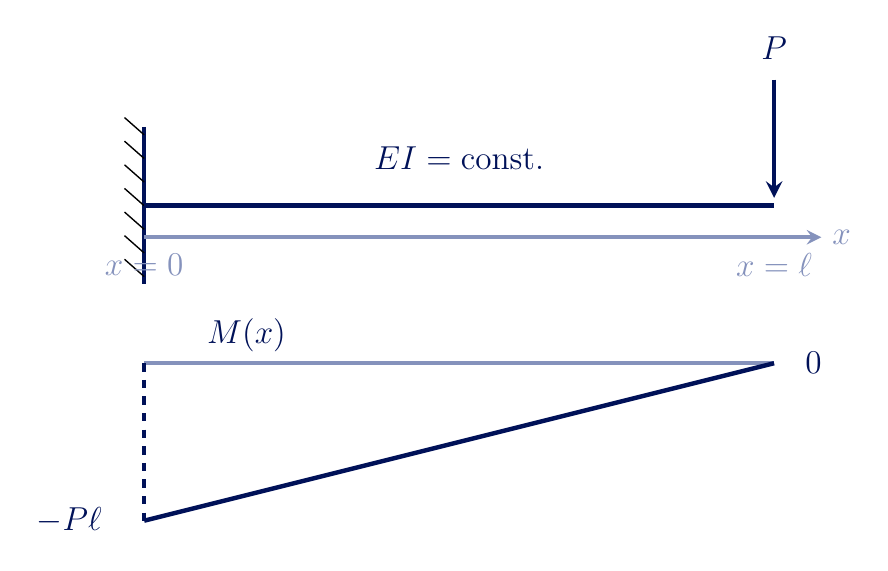
\begin{tikzpicture}[>=stealth, line width=1.3pt, font=\large]
  % wall / fixed support
  \draw[mainblue, line width=1.5pt] (0,1.0) -- (0,-1.0);
  \foreach \y in {-0.9,-0.6,...,0.9} {
    \draw[line width=0.5pt] (0,\y) -- (-0.25,\y+0.22);
  }

  % beam
  \draw[mainblue, line width=2pt] (0,0) -- (8,0);

  % coordinate x
  \draw[accent, ->] (0,-0.4) -- (8.6,-0.4) node[right] {$x$};
  \node[accent] at (0,-0.75) {$x=0$};
  \node[accent] at (8,-0.75) {$x=\ell$};

  % load P at free end
  \draw[mainblue, ->, line width=1.6pt] (8,1.6) -- (8,0.1);
  \node[mainblue] at (8,2.0) {$P$};

  \node[mainblue] at (4,0.6) {$EI = \text{const.}$};

  % moment diagram below: max magnitude at the wall (x=0), zero at the free end (x=l)
  \draw[accent] (0,-2.0) -- (8,-2.0);
  \draw[mainblue, line width=1.6pt] (0,-4.0) -- (8,-2.0);
  \draw[mainblue, dashed] (0,-2.0) -- (0,-4.0);
  \node[mainblue] at (1.3,-1.65) {$M(x)$};
  \node[mainblue] at (-0.95,-4.0) {$-P\ell$};
  \node[mainblue] at (8.5,-2.0) {$0$};
\end{tikzpicture}

% ---------- PAGE 2: Einfeldtraeger with point load F at midspan ----------
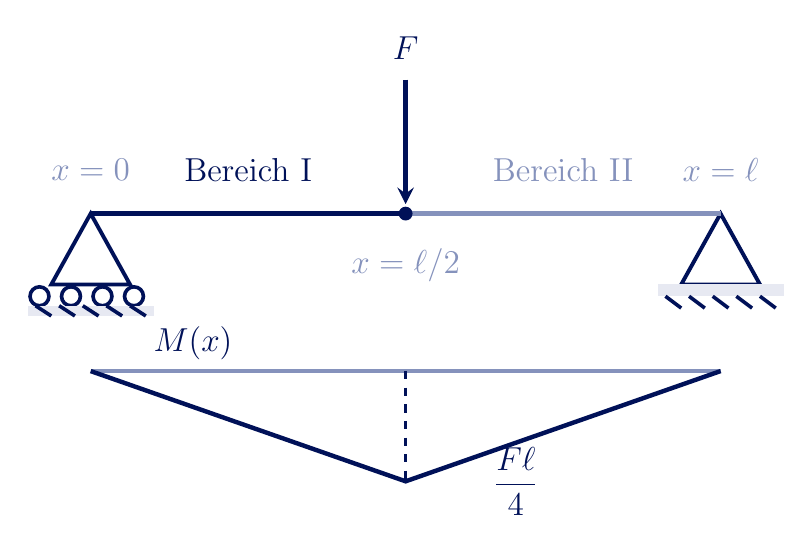
\begin{tikzpicture}[>=stealth, line width=1.3pt, font=\large]
  % roller support left (Loslager)
  \draw[mainblue, line width=1.4pt] (0,0) -- (-0.5,-0.9) -- (0.5,-0.9) -- cycle;
  \draw[mainblue] (-0.65,-1.05) circle (0.12);
  \draw[mainblue] (-0.25,-1.05) circle (0.12);
  \draw[mainblue] (0.15,-1.05) circle (0.12);
  \draw[mainblue] (0.55,-1.05) circle (0.12);
  \fill[lightaccent] (-0.8,-1.3) rectangle (0.8,-1.17);
  \foreach \x in {-0.7,-0.4,...,0.7} {
    \draw[mainblue] (\x,-1.17) -- (\x+0.2,-1.3);
  }

  % pin support right (Festlager)
  \draw[mainblue, line width=1.4pt] (8,0) -- (7.5,-0.9) -- (8.5,-0.9) -- cycle;
  \fill[lightaccent] (7.2,-0.9) rectangle (8.8,-1.05);
  \foreach \x in {7.3,7.6,...,8.7} {
    \draw[mainblue] (\x,-1.05) -- (\x+0.2,-1.2);
  }

  % beam, split into region I and II
  \draw[mainblue, line width=2pt] (0,0) -- (4,0);
  \draw[accent, line width=2pt] (4,0) -- (8,0);
  \fill[mainblue] (4,0) circle (2.5pt);

  \node[mainblue] at (2.0,0.55) {Bereich I};
  \node[accent] at (6.0,0.55) {Bereich II};

  % load F at midspan
  \draw[mainblue, ->, line width=1.6pt] (4,1.7) -- (4,0.12);
  \node[mainblue] at (4,2.1) {$F$};

  % coordinate
  \node[accent] at (0,0.55) {$x=0$};
  \node[accent] at (8,0.55) {$x=\ell$};
  \node[accent] at (4,-0.65) {$x=\ell/2$};

  % moment diagram (triangular)
  \draw[accent] (0,-2.0) -- (8,-2.0);
  \draw[mainblue, line width=1.6pt] (0,-2.0) -- (4,-3.4) -- (8,-2.0);
  \draw[mainblue, dashed] (4,-2.0) -- (4,-3.4);
  \node[mainblue] at (1.3,-1.65) {$M(x)$};
  \node[mainblue] at (5.4,-3.4) {$\dfrac{F\ell}{4}$};
\end{tikzpicture}

% ---------- PAGE 3: Kragarm - Biegelinie w(x) ----------
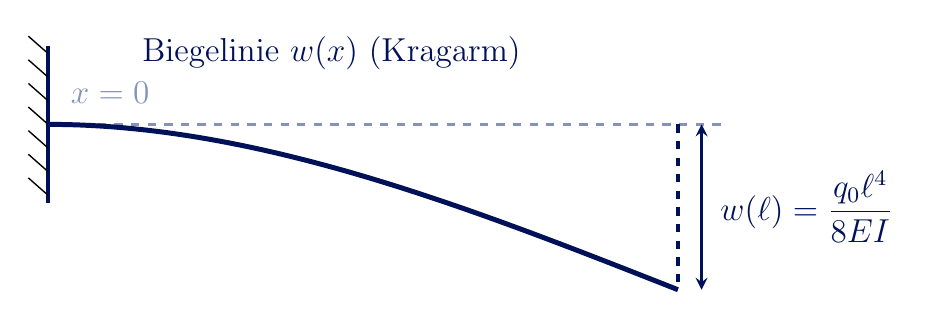
\begin{tikzpicture}[>=stealth, line width=1.3pt, font=\large]
  % wall / fixed support
  \draw[mainblue, line width=1.5pt] (0,1.0) -- (0,-1.0);
  \foreach \y in {-0.9,-0.6,...,0.9} {
    \draw[line width=0.5pt] (0,\y) -- (-0.25,\y+0.22);
  }

  % undeformed reference line
  \draw[accent, dashed, line width=0.9pt] (0,0) -- (8.6,0);

  % deflection curve w(x) = -(3/2)xi^2 + (1/2)xi^3, xi=x/l, scaled
  \draw[mainblue, line width=1.8pt]
    plot[domain=0:8,samples=60] (\x,{-2.1*(1.5*(\x/8)*(\x/8) - 0.5*(\x/8)*(\x/8)*(\x/8))});

  \draw[mainblue, dashed] (8,0) -- (8,-2.1);
  \draw[mainblue, <->, line width=0.9pt] (8.3,0) -- (8.3,-2.1);
  \node[mainblue, anchor=west] at (8.4,-1.05) {$w(\ell)=\dfrac{q_0\ell^4}{8EI}$};

  \node[accent, anchor=west] at (0.15,0.4) {$x=0$};
  \node[mainblue] at (3.6,0.9) {Biegelinie $w(x)$ (Kragarm)};
\end{tikzpicture}

% ---------- PAGE 4: Einfeldtraeger - Biegelinie w(x) ----------
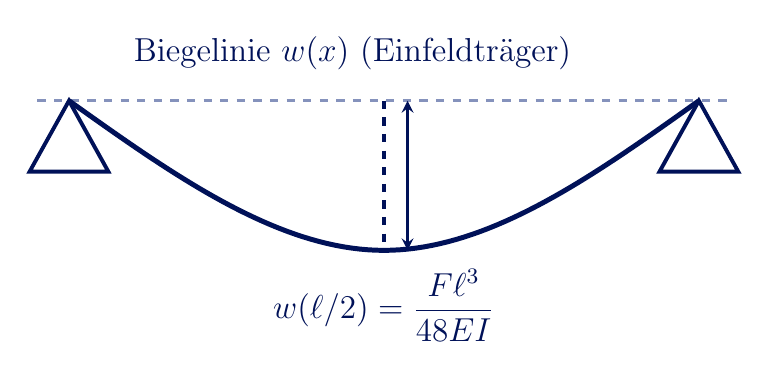
\begin{tikzpicture}[>=stealth, line width=1.3pt, font=\large]
  % roller support left
  \draw[mainblue, line width=1.4pt] (0,0) -- (-0.5,-0.9) -- (0.5,-0.9) -- cycle;
  % pin support right
  \draw[mainblue, line width=1.4pt] (8,0) -- (7.5,-0.9) -- (8.5,-0.9) -- cycle;

  % undeformed reference line
  \draw[accent, dashed, line width=0.9pt] (-0.4,0) -- (8.4,0);

  % deflection curve, symmetric: w(x)=-(3 xi - 4 xi^3) on [0,l/2], mirrored on [l/2,l], xi=x/l
  \draw[mainblue, line width=1.8pt]
    plot[domain=0:4,samples=40] (\x,{-1.9*(3*(\x/8) - 4*(\x/8)*(\x/8)*(\x/8))});
  \draw[mainblue, line width=1.8pt]
    plot[domain=4:8,samples=40] (\x,{-1.9*(3*((8-\x)/8) - 4*((8-\x)/8)*((8-\x)/8)*((8-\x)/8))});

  \draw[mainblue, dashed] (4,0) -- (4,-1.9);
  \draw[mainblue, <->, line width=0.9pt] (4.3,0) -- (4.3,-1.9);
  \node[mainblue, align=center] at (4,-2.6) {$w(\ell/2)=\dfrac{F\ell^3}{48EI}$};

  \node[mainblue] at (3.6,0.6) {Biegelinie $w(x)$ (Einfeldträger)};
\end{tikzpicture}

% ---------- PAGE 5: Uebergangsbedingung - Ausblick-Skizze ----------
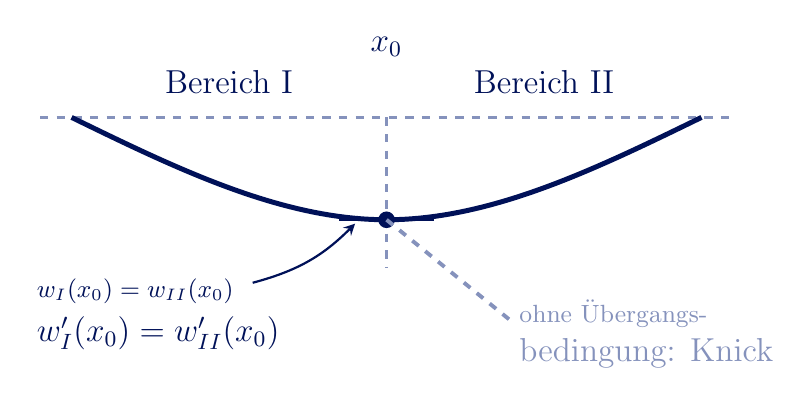
\begin{tikzpicture}[>=stealth, line width=1.3pt, font=\large]
  % reference axis (undeformed beam)
  \draw[accent, dashed, line width=0.9pt] (-0.4,0) -- (8.4,0);

  % Bereich labels
  \node[mainblue] at (2.0,0.45) {Bereich I};
  \node[mainblue] at (6.0,0.45) {Bereich II};
  \node[mainblue] at (4,0.9) {$x_0$};
  \draw[accent, dashed] (4,0) -- (4,-1.9);

  % correct, smooth deflection curve (continuous w and w')
  \draw[mainblue, line width=1.8pt]
    plot[domain=0:4,samples=40] (\x,{-1.3*(3*(\x/8) - 4*(\x/8)*(\x/8)*(\x/8))});
  \draw[mainblue, line width=1.8pt]
    plot[domain=4:8,samples=40] (\x,{-1.3*(3*((8-\x)/8) - 4*((8-\x)/8)*((8-\x)/8)*((8-\x)/8))});

  % horizontal tangent at the junction, to show the slope really is continuous
  \draw[mainblue, line width=0.6pt] (3.4,-1.3) -- (4.6,-1.3);
  \fill[mainblue] (4,-1.3) circle (3pt);

  % wrong continuation without matching slope -> visible kink
  \draw[accent, dashed, line width=1.4pt] (4,-1.3) -- (5.6,-2.6);
  \node[accent, align=left] at (7.3,-2.75) {\small ohne Übergangs-\\bedingung: Knick};

  % callout for the correct, smooth join
  \node[mainblue, align=left] at (1.1,-2.5) {\small $w_I(x_0)=w_{II}(x_0)$\\[2pt] $w_I'(x_0)=w_{II}'(x_0)$};
  \draw[mainblue, ->, line width=0.8pt] (2.3,-2.1) to[bend right=15] (3.6,-1.35);
\end{tikzpicture}

\end{document}
